%%%%%%%%%%%%%%%%%%%%%%%%%%%%%%%%%%%%%%%%%%%%%%%%%%%%%%%%%%%%%%%%%%%%%%%%%%%%%%%
%% Appendix
%%%%%%%%%%%%%%%%%%%%%%%%%%%%%%%%%%%%%%%%%%%%%%%%%%%%%%%%%%%%%%%%%%%%%%%%%%%%%%%

\appendix

%%%%%%%%%%%%%%%%%%%%%%%%%%%%%%%%%%%%%%%%%%%%%%%%%%%%%%%%%%%%%%%%%%%%%%%%%%%%%%%
%%
%% Beispiel Datenbank
%%
%%%%%%%%%%%%%%%%%%%%%%%%%%%%%%%%%%%%%%%%%%%%%%%%%%%%%%%%%%%%%%%%%%%%%%%%%%%%%%%
\chapter{Beispiel Datenbank-Schema} \label{beispiel-datenbankschema}

\begin{figure}[htbp]
  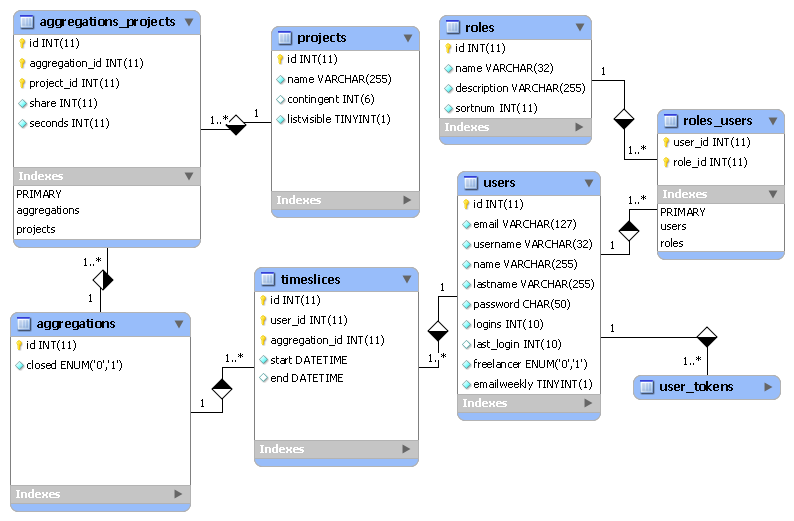
\includegraphics[width=\textwidth]{figures/beispiel-datenbankschema}
  \caption{Die Beispieldatenbank}
  \label{beispiel-datenbankschema-bild}
\end{figure}

\noindent Das Schema modelliert eine Applikation um die Arbeitszeiten von Mitarbeiten zu bestimmen. In \tabelle{timeslices} sind dabei Zeitspannen, die der Benutzer im Betrieb gearbeitet hat. Er loggt sich morgens ein und Abends wieder aus. Nach dem Arbeitstag erstellt er eine Aggregation. Eine Aggregation kann mehrere Timeslices besitzen und wird Projekten zugeordnet. Es wird dann die Zeit in einer Aggregation, die von den Timeslices kommt, auf die zugeordneten Projekte verteilt. \\
\\
\label{beispiel-datenbank-kardinalitaeten}
\begin{tabular}{|l|c|} 
\hline
Relation & Anzahl der Zeilen \\
\hline
\tabelle{projects} & 193 \\
\hline
\tabelle{aggregations\_projects} & 11.862\\
\hline
\tabelle{aggregations} & 3.742\\
\hline
\tabelle{timeslices} & 4.151\\
\hline
\tabelle{users} & 20\\
\hline
\end{tabular}


%%%%%%%%%%%%%%%%%%%%%%%%%%%%%%%%%%%%%%%%%%%%%%%%%%%%%%%%%%%%%%%%%%%%%%%%%%%%%%%
%%
%% Evaluation
%%
%%%%%%%%%%%%%%%%%%%%%%%%%%%%%%%%%%%%%%%%%%%%%%%%%%%%%%%%%%%%%%%%%%%%%%%%%%%%%%%
\chapter{Quelltext der Evaluation} \label{tests-code}


%%%%%%%%%%%%%%%% DOCTRINE  %%%%%%%%%%%%%%%%
\begin{fcode}
    \lstset{style=php}
    \begin{lstlisting}
// [...] bootstrap

$em->getRepository('Entities\Project')->findAll();
$em->getRepository('Entities\Aggregation')->findAll();
$objects = $em->getRepository('Entities\Aggregation2Project')->findAll();

?>
<html><head><title>Doctrine Test1</title></head>

<body>
<?php include 'print_objects.php'; ?>
</body>

</html>
    \end{lstlisting}
    \caption{Doctrine Test1}
\end{fcode}


\begin{fcode}
    \lstset{style=php}
    \begin{lstlisting}
// [...] bootstrap

$query = $em->createQuery("SELECT a2p, p, a FROM Aggregation2Project a2p JOIN a2p.project p JOIN a2p.aggregation a ORDER BY a2p.id");
$objects = $query->getResult();

?>
<html><head><title>Doctrine Test2</title></head>

<body>
<?php include 'print_objects.php'; ?>
</body>

</html>
    \end{lstlisting}
    \caption{Doctrine Test1}
\end{fcode}

%%%%%%%%%%%%%%%% KOHANA %%%%%%%%%%%%%%%%
\begin{fcode}
    \lstset{style=php}
    \begin{lstlisting}
// Code im Controller

$objects = ORM::factory('Aggregations_Project')->find_all();

?>
<html><head><title>Kohana Test1</title></head>

<body>
<?php include 'print_objects.php'; ?>
</body>

</html>
    \end{lstlisting}
    \caption{Kohana Test1}
\end{fcode}


\begin{fcode}
    \lstset{style=php}
    \begin{lstlisting}
// Code im Controller

$objects = ORM::factory('Aggregations_Project')
    ->with('project')
    ->with('aggregation')
    ->find_all();
?>
<html><head><title>Kohana Test2</title></head>

<body>
<?php include 'print_objects.php'; ?>
</body>

</html>
    \end{lstlisting}
    \caption{Kohana Test2}
\end{fcode}


%%%%%%%%%%%%%%% PSCORM %%%%%%%%%%%%%%%%%%%%%%

\begin{fcode}
    \lstset{style=php}
    \begin{lstlisting}
// Code im Controller

$q = new PScorm_QueryTest1($db);
$objects = $q->getAllAggregation2Project();


?><html><head><title>PSCORM Test1</title></head>

<body>
<?php include 'print_objects.php'; ?>
</body>

</html>

// QueryTest1 Class
public function getAllAggregation2Project() {
  $this->getAll('Project');
  $this->getAll('Aggregation');
  
  return $this->getAll('Aggregation2Project',' ORDER BY aggregations_projects.id');
}

public function getAll($class, $orderbySQL = NULL) {
  $class = 'PScorm_'.$class;
  $o = new $class;
  
  $sql = "SELECT * FROM ".$o->getTable().$orderbySQL;
  
  $ret = array();
  $cache = PScorm_Cache::instance();
  foreach ($this->fetchResult($sql) as $row) {
    $o = new $class();
    $o->result = $row;
    $o->init();
    
    $cache->populate($o);
    $ret[] = $o;
  }
  return $ret;
}
    \end{lstlisting}
    \caption{PSCORM Test1}
\end{fcode}


\begin{fcode}
    \lstset{style=php}
    \begin{lstlisting}
// Code im Controller

$q = new PScorm_QueryTest2($db);
$objects = $q->getAllAggregation2Project();

?><html><head><title>PSCORM Test2</title></head>

<body>
<?php include 'print_objects.php'; ?>
</body>

</html>

    \end{lstlisting}
    \caption{PSCORM Test2}
\end{fcode}



\begin{fcode}
    \lstset{style=php}
    \begin{lstlisting}
public function getAllAggregation2Project() {
  $o = new PScorm_Aggregation2Project;

  // SQL fuer die JOIN Abfrage
  $sql = "SELECT aggregations_projects.*,
              aggregations.id as aggregations_id,
              aggregations.closed as aggregations_closed,
              projects.id as projects_id,
              projects.name as projects_name,
              projects.contingent as projects_contingent,
              projects.listvisible as projects_listvisible ";
  $sql .= "FROM ".$o->getTable()." ";
  $sql .= SQL::LEFTJOIN('aggregations',array($o->getTable(),'id','aggregation_id'),'1:n');
  $sql .= SQL::LEFTJOIN('projects',array($o->getTable(),'id','project_id'),'1:n');
  
  $ret = array();
  $cache = PScorm_Cache::instance();
  foreach ($this->fetchResult($sql) as $row) {
  
    //Aggregation-Objekt laden und Ergebnis aus der Datenbankzeile uebergeben
    $a = new PScorm_Aggregation;
    $a->result = $row;
    $a->prefix = 'aggregations_';
    $a->init();
    $cache->populate($a);
    
    //Project-Objekt laden und Ergebnis aus der Datenbankzeile uebergeben
    $p = new PScorm_Project;
    $p->result = $row;
    $p->prefix = 'projects_';      
    $p->init();
    $cache->populate($p);
    
    //Gesamtobjektladen
    $o = new PScorm_Aggregation2Project;
    $o->result = $row;
    $o->init();
    $cache->populate($o);
    
    // dem Ergebnis hinzufuegen
    $ret[] = $o;
  }
  return $ret;
}
    \end{lstlisting}
    \caption{PSCORM Test2: QueryTest2 Klasse}
\end{fcode}

%%%%%%%%%%%%%%%%%%%%%%%%%%%%%%%%%%%%%%%%%%%%%%%%%%%%%%%%%%%%%%%%%%%%%%%%%%%%%%%
%%
%% Correspondence
%%
%%%%%%%%%%%%%%%%%%%%%%%%%%%%%%%%%%%%%%%%%%%%%%%%%%%%%%%%%%%%%%%%%%%%%%%%%%%%%%%
%\chapter{Correspondence}

\chapter{Implementierungsübersicht PSCORM}

Hier wird die Struktur der \PSCORM-Demoapplikation vorgestellt um eine Übersicht zu erhalten. Die Quelltexte der Demoapplikation befinden sich auf Github:
\begin{verbatim}
https://github.com/pscheit/Diplomarbeit
\end{verbatim}
\noindent Die wichtigen Auszüge dieser Quelltexte wurden schon in Anhang \ref{tests-code} aufgelistet. \\
In \texttt{htdocs/pscorm} sind alle Klassen für die Demoapplikation. Diese Klassenstruktur sieht genauso aus, wie ein Export von \PSCORM in Zukunft aussehen soll. Es lassen sich keine komplexen Klassen, oder große Ordnerstrukturen finden. \\
Zusätzlich liegen in \texttt{htdocs/doctrine} und \texttt{htdocs/kohana} die Quelltexte für die Tests in Kapitel \ref{evaluation}. In \texttt{htdocs/kohana} sind die Klassen und Libraries von Kohana direkt enthalten. In \texttt{htdocs/doctrine} befinden sich nur die Controller, die Sourcen befinden sich in \texttt{../inc/doctrine/-orm/Doctrine}. Die Abhängigkeiten von \PSCORM zum Psc-Framework wurden nicht aufgelöst. \\
\\
Alle Pfade die ich jetzt nenne sind relativ zu \texttt{htdocs/pscorm}. \\
\subsubsection{inc.config.php}
Für das übergeordnete Psc-Framework werden hier die Zugangsdaten für die Datenbank und die Datenbank angegeben. Das Schema der Datenbank befindet sich in \texttt{../../schema.sql}

\subsubsection{class}
Im Verzeichnis befinden sich alle Klassen der Demoapplikation. Alle Klassen haben den Prefix \texttt{PScorm\_}, damit sie unterscheidbar bleiben. Diese sollten mit einem PHP-Autoloader dynamisch geladen werden. Fast alle Klassen leiten \code{Object} ab. Diese kann als Basisklasse des Psc-Frameworks verstanden werden.

\subsubsection{DB.php}
Die Klasse mit der native Anfragen an die konfigurierte Datenbank abgesetzt werden können. Leitet PDO ab, welches eine in die Pecl-Extension PDO (\url{http://www.php.net/PDO}) eingebaute Klasse ist. Die funktion \code{query()} wurde dabei überschrieben, so dass alle SQL Befehle aus der Applikation in das Logfile gesichert werden können. Das Logfile kann dann zum Debug gebraucht werden (siehe \code{\_\_toString()}).

\subsubsection{Cache.php}
Die Klasse für den Cache. Ist als Singleton implementiert und kann von überall mit \code{PScorm\_Cache::getInstance()} geladen werden.

\subsubsection{ORMObject.php}
Die abstrakte Basisklasse für alle Entity-Klassen (Project, Aggregation2Project, Aggregation). Sie stellt die wichtige Funktion \code{PScorm\_ORMObject::load}, die immer in der Applikation aufgerufen wird, wenn ein Objekt aus der Datenbank geladen werden soll. \\
Die Abstrakte Funktion \code{init()} muss von allen Entity-Klassen implementiert werden. Der Datensatz aus der Datenbank wird im Property \code{result} gespeichert.

\subsubsection{Query.php}
Die Basisklasse für alle Queries. Stellt \code{getAll()} zur Verfügung, welche z.~B. in Query1 benutzt wird.

\subsubsection{Query[0-9].php}
Die Query-Klassen für die verschiedenen Tests. Leiten die Klasse Query ab.

\subsubsection{Project.php Aggregation.php Aggregation2Project.php}
Entity-Klassen für Project Aggregation und Aggregation2Project. Aggregation2Project benutzt die \code{load()}-Funktion von ORMObject um seine Unterobjekte zu initialisieren.

%%%%%%%%%%%%%%%%%%%%%%%%%%%%%%%%%%%%%%%%%%%%%%%%%%%%%%%%%%%%%%%%%%%%%%%%%%%%%%%
%%
%% Correspondence
%%
%%%%%%%%%%%%%%%%%%%%%%%%%%%%%%%%%%%%%%%%%%%%%%%%%%%%%%%%%%%%%%%%%%%%%%%%%%%%%%%
%\chapter{Correspondence}

%%%%%%%%%%%%%%%%%%%%%%%%%%%%%%%%%%%%%%%%%%%%%%%%%%%%%%%%%%%%%%%%%%%%%%%%%%%%%%%
%%
%% Keyword Index
%%
%%%%%%%%%%%%%%%%%%%%%%%%%%%%%%%%%%%%%%%%%%%%%%%%%%%%%%%%%%%%%%%%%%%%%%%%%%%%%%%
%\addcontentsline{toc}{chapter}{Index}
%\printindex
%\newpage


%%%%%%%%%%%%%%%%%%%%%%%%%%%%%%%%%%%%%%%%%%%%%%%%%%%%%%%%%%%%%%%%%%%%%%%%%%%%%%%
%%
%% Bibliography
%%
%%%%%%%%%%%%%%%%%%%%%%%%%%%%%%%%%%%%%%%%%%%%%%%%%%%%%%%%%%%%%%%%%%%%%%%%%%%%%%%

%% ENGLISH:
%  \addcontentsline{toc}{chapter}{Bibliography}
\addcontentsline{toc}{chapter}{Literaturverzeichnis}
\bibliographystyle{alpha}
\bibliography{thesis}
